\chapter{Grundbegriffe}

F\"{u}r das Verst\"{a}ndnis wie die Simulation von verteilten Systemen funktioniert, werden hier einige Grundbegriffe erl\"{a}utert. Eine Vertiefung findet erst in den nachfolgenden Kapiteln statt.

\section{Client/Server Modell}

Der Simulator basiert auf dem Client/Server Prinzip. Bei jeder sinnvollen Simulation gibt es mindestens einen teilnehmenden Client und einen Server, die miteinander \"{u}ber Nachrichten (s.u.) kommunizieren (Abbildung \ref{fig:ClientServer}). Bei komplexen Simulationen k\"{o}nnen auch mehrere Clients und/oder Server mitwirken. In der Regel empfangen Server nur Nachrichten, die von Clients verschickt wurden und virce versa.

\begin{figure}[htbp]
	\centering
	\fbox{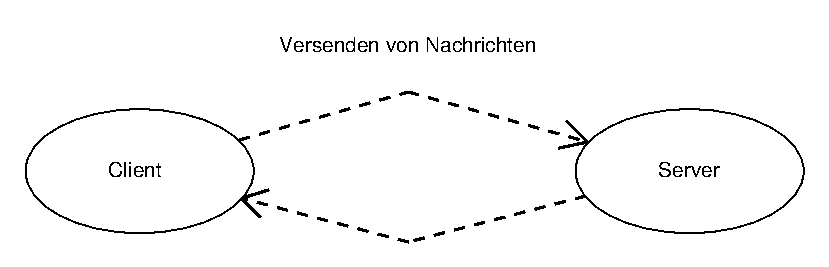
\includegraphics{images/client-server}}
	\caption{Client/Server Modell}
	\label{fig:ClientServer}
\end{figure}

\section{Prozesse und deren Rollen}

Ein verteiltes System wird anhand von Prozessen simuliert. Jeder Prozess nimmt hierbei eine oder mehrere Rollen ein. Beispielsweise kann ein Prozess die Rolle eines Clients einnehmen und ein weiterer Prozess die Rolle eines Servers. Ein Prozess kann auch Client und Server gleichzeitig sein. Es ist auch m\"{o}glich, dass ein Prozess die Rollen mehrerer Server und Clients aufeinmal einnimmt. Ob das sinnvoll ist h\"{a}ngt vom Szenario ab. Um einen Prozess zu kennzeichnen besitzt jeder Prozess eine \textbf{eindeutige} Prozess-Identifikationsnummer (PID).

\section{Nachrichten}

Damit das Client/Server Modell angewandt werden kann, m\"{u}ssen Nachrichten verschickt werden k\"{o}nnen. Eine Nachricht kann von einem Client- oder Serverprozess verschickt werden und kann beliebig viele Empf\"{a}nger haben. Der Inhalt einer Nachricht h\"{a}ngt vom verwendeten Protokoll (s.u.) ab. Um eine Nachricht zu kennzeichnen besitzt jede Nachricht eine \textbf{eindeutige} Nachrichten-Identifikationsnummer (NID).

\section{Lokale und globale Uhren}

In einer Simulation gibt es \textbf{genau eine} globale Uhr. Sie stellt die aktuelle und \textbf{immer korrekte} Zeit dar. Eine globale Uhr geht nie falsch.

Zudem besitzt jeder beteiligter Prozess eine eigene lokale Uhr. Sie stellt die aktuelle, jedoch nicht zwangsm\"{a}�ig global-korrekte, Zeit des jeweiligen Prozesses dar. Wenn die Prozesszeit nicht korrekt ist (nicht der globalen Zeit gleicht), dann wurde die Prozessuhr entweder im Laufe einer Simulation neugestellt oder sie besitzt eine Uhrabweichung. Eine Uhrabweichung gibt an, um wieviel eine Uhr falsch geht. Wenn eine lokale Uhr nicht neugesetzt wird und auch keine Uhrabweichung hat, dann gibt sie stets die korrekte globale Zeit wieder. 

\section{Ereignisse}

Eine Simulation besteht aus der Hintereinanderausf\"{u}hrung von endlich vielen Ereignissen. Beispielsweise kann es ein Ereignis geben, welches einen Prozess eine Nachricht verschicken l\"{a}�t oder den Prozess selbst abst\"{u}rzen l\"{a}�t. Jedes Ereignis tritt zu einem bestimmten Zeitpunkt ein. Wenn es zeitgleiche Ereignisse gibt, so werden sie ebenso hintereinander ausgef\"{u}hrt, behalten aber in der Simulation die selben Ausf\"{u}hrzeiten.

\section{Protokolle}

\begin{figure}[htbp]
	\centering
	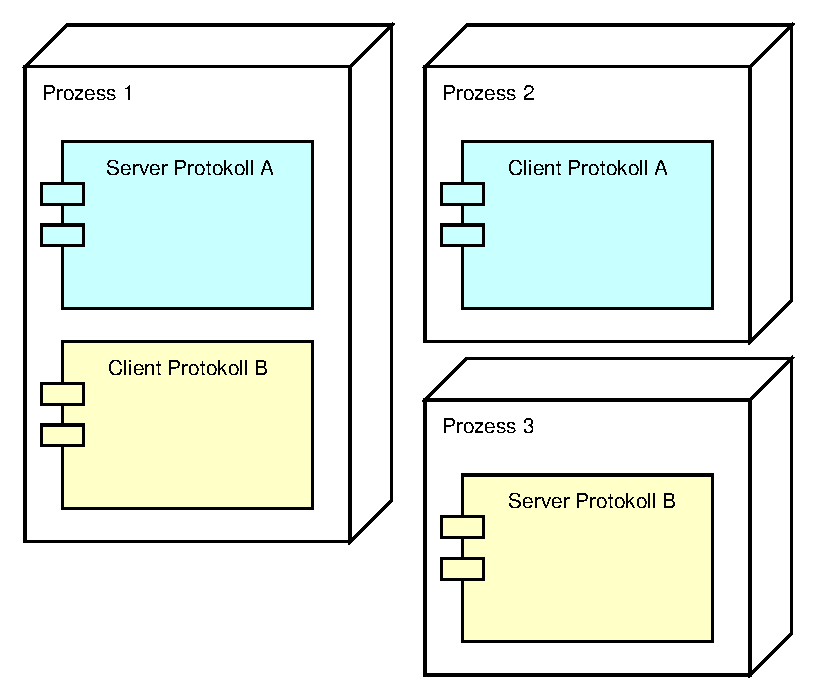
\includegraphics{images/client-server-protokolle}
	\caption{Client/Server Protokolle}
	\label{fig:ClientServerProtokolle}
\end{figure}

Eine Simulation besteht aus der Anwendung von Protokollen. Es wurde bereits erw\"{a}hnt, dass ein Prozess die Rollen von Servern und/oder Clients annehmen kann. Bei jeder Server- und Clientrolle muss zus\"{a}tzlich das dazugeh\"{o}rige Protokoll spezifiziert werden. Ein Protokoll definiert, wie ein Client und ein Server Nachrichten verschicken und wie sie bei Ankunft von Nachrichten reagieren. Ein Prozess verarbeitet eine empfangene Nachricht nur, wenn er das jeweilige Protokoll versteht.

In Abbildung \ref{fig:ClientServerProtokolle} sind 3 Prozesse dargestellt. Prozess 1 unterst\"{u}tzt serverseitig das Protokoll ``A'' und clientseitig das Protokoll ``B''. Prozess 2 unterst\"{u}tzt clientseitig das Protokoll ``A'' und Prozess 3 serverseitig das Protokoll ``B''. D.h., Prozess 1 kann mit Prozess 2 via Protokoll ``A'' und mit Prozess 3 via Protokoll ``B'' kommunizieren. Die Prozesse 2 und 3 sind zueinander inkompatibel.
